
\chapter{Architekturübersicht}
\label{chap:architektur}

\section{Gesamtarchitektur}

Die entwickelte Lösung basiert auf einer mehrstufigen Architektur, die aus Retrieval-, Feature-Engineering- und Ranking-Komponenten besteht. 
Im Gegensatz zu klassischen Suchsystemen, bei denen auf eine Anfrage direkte Ergebnisse gerankt werden, wird in diesem System ein anderer Ansatz verwendet.
Dabei werden mehrere Retrievalsignale erzeugt, die im Anschluss zusammen mit technischen Merkmalen als Eingabe für das Learning-to-Rank-Modell verwendet werden.

Die einzelnen Schritte der Pipeline reichen von der Datenaufbereitung, über die Kandidatenbildung bis hin zum modellbasierten Ranking.

Abbildung \ref{fig:architektur} zeigt die implementierte End-to-End-Pipeline des Systems.

\usetikzlibrary{positioning, arrows.meta}

\begin{figure}[htbp]
    \centering
    \resizebox{!}{0.68\textheight}{%
    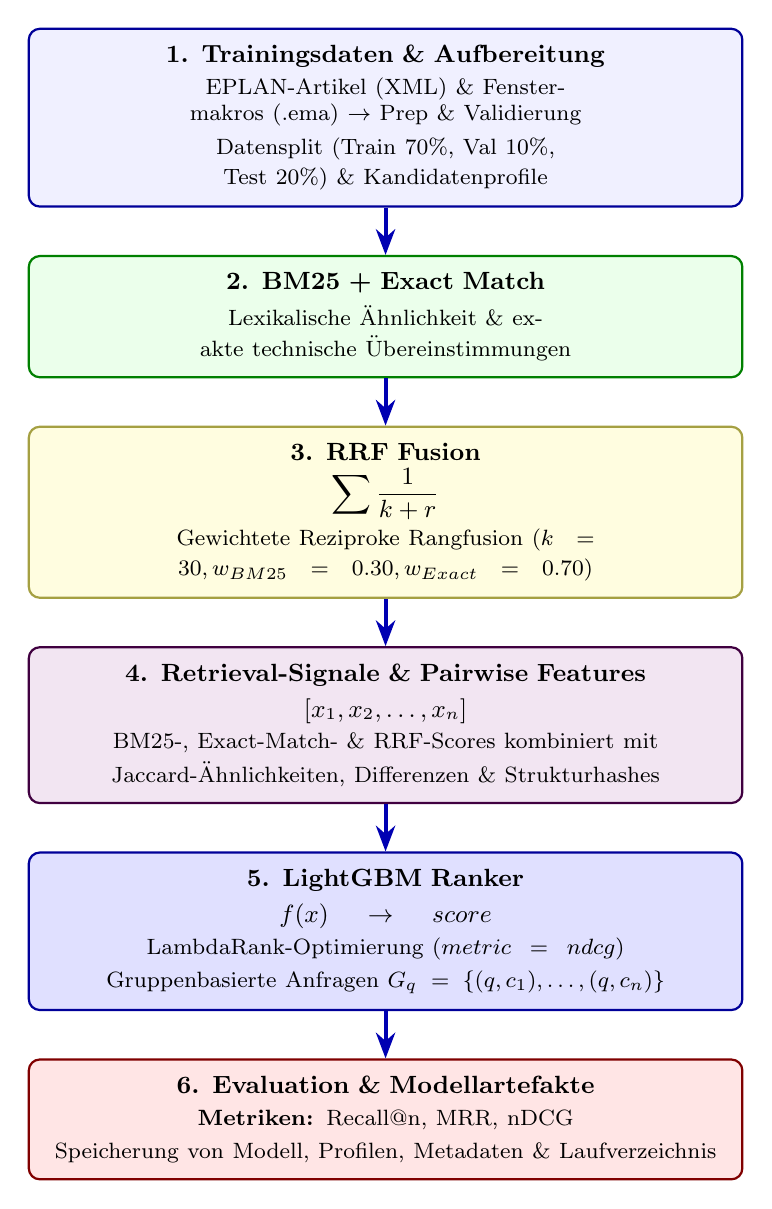
\begin{tikzpicture}[
        >=Stealth,
        font=\small,
        databox/.style={draw=blue!60!black, thick, rounded corners=4pt, fill=blue!6, text width=8.5cm, minimum height=1.2cm, align=center, inner ysep=6pt, inner xsep=8pt},
        retbox/.style={draw=green!50!black, thick, rounded corners=4pt, fill=green!8, text width=8.5cm, minimum height=1.1cm, align=center, inner ysep=6pt, inner xsep=8pt},
        fusionbox/.style={draw=yellow!60!black, thick, rounded corners=4pt, fill=yellow!12, text width=8.5cm, minimum height=1.2cm, align=center, inner ysep=6pt, inner xsep=8pt},
        featurebox/.style={draw=violet!50!black, thick, rounded corners=4pt, fill=violet!10, text width=8.5cm, minimum height=1.3cm, align=center, inner ysep=6pt, inner xsep=8pt},
        modelbox/.style={draw=blue!60!black, thick, rounded corners=4pt, fill=blue!12, text width=8.5cm, minimum height=1.3cm, align=center, inner ysep=6pt, inner xsep=8pt},
        evalbox/.style={draw=red!50!black, thick, rounded corners=4pt, fill=red!10, text width=8.5cm, minimum height=1.2cm, align=center, inner ysep=6pt, inner xsep=8pt},
        flow/.style={->, >=Stealth, line width=1.4pt, blue!70!black}
    ]
        % Block 1: Trainingsdaten
        \node[databox] (data) {
            \textbf{1. Trainingsdaten \& Aufbereitung}\\[2pt]
            \footnotesize EPLAN-Artikel (XML) \& Fenstermakros (.ema) $\rightarrow$ Prep \& Validierung\\[1pt]
            Datensplit (Train 70\%, Val 10\%, Test 20\%) \& Kandidatenprofile
        };

        % Block 2: BM25 + Exact Match
        \node[retbox, below=0.6cm of data] (retrieval) {
            \textbf{2. BM25 + Exact Match}\\[2pt]
            \footnotesize Lexikalische Ähnlichkeit \& exakte technische Übereinstimmungen
        };

        % Block 3: RRF Fusion
        \node[fusionbox, below=0.6cm of retrieval] (rrf) {
            \textbf{3. RRF Fusion}\\[2pt]
            \small $\displaystyle \sum \frac{1}{k + r}$\\[2pt]
            \footnotesize Gewichtete Reziproke Rangfusion ($k=30, w_{\text{BM25}}=0.30, w_{\text{Exact}}=0.70$)
        };

        % Block 4: Retrieval-Signale als Features
        \node[featurebox, below=0.6cm of rrf] (features) {
            \textbf{4. Retrieval-Signale \& Pairwise Features}\\[2pt]
            \small $[x_1, x_2, \dots, x_n]$\\[2pt]
            \footnotesize BM25-, Exact-Match- \& RRF-Scores kombiniert mit\\[1pt]
            Jaccard-Ähnlichkeiten, Differenzen \& Strukturhashes
        };

        % Block 5: LightGBM Ranker
        \node[modelbox, below=0.6cm of features] (ranker) {
            \textbf{5. LightGBM Ranker}\\[2pt]
            \small $f(x) \rightarrow \text{score}$\\[2pt]
            \footnotesize LambdaRank-Optimierung ($\text{metric}=\text{ndcg}$)\\[1pt]
            Gruppenbasierte Anfragen $G_q = \{(q,c_1),\dots,(q,c_n)\}$
        };

        % Block 6: Evaluation
        \node[evalbox, below=0.6cm of ranker] (eval) {
            \textbf{6. Evaluation \& Modellartefakte}\\[2pt]
            \footnotesize \textbf{Metriken:} Recall@n, MRR, nDCG\\[1pt]
            Speicherung von Modell, Profilen, Metadaten \& Laufverzeichnis
        };

        % Verbindungen (Ablaufkette von 1 -> 2 -> 3 -> 4 -> 5 -> 6)
        \draw[flow] (data.south) -- (retrieval.north);
        \draw[flow] (retrieval.south) -- (rrf.north);
        \draw[flow] (rrf.south) -- (features.north);
        \draw[flow] (features.south) -- (ranker.north);
        \draw[flow] (ranker.south) -- (eval.north);
    \end{tikzpicture}%
    }
    \caption{Architektur der Trainings- und Rankingpipeline.}
    \label{fig:architektur}
\end{figure}


Die Orchestrierung aller Verarbeitungsschritte erfolgt zentral über die Trainingspipeline \cite{srcPipeline}.